\documentclass[aspectratio=169]{beamer}
\usetheme{Boadilla} % plainest one with slide number footer

% generic packages

\usepackage[utf8]{inputenc}
\usepackage[english]{babel}
\usepackage{amsmath}
\usepackage{multicol}
\usepackage{ulem}
\usepackage{tikz}

\tikzset{
	proto/.style = {shape=rectangle, rounded corners, draw, align=center, fill=green!30},
	res/.style = {shape=rectangle, rounded corners, draw, align=center, fill=blue!30},
	nonres/.style = {shape=rectangle, rounded corners, draw, align=center, color=black!50, fill=blue!10},
	host/.style = {shape=rectangle, rounded corners, draw, align=center, fill=gray!30},
	req/.style = {shape=rectangle, draw, align=left},
}

% about the presentation
\title{CoAP Protocol Indication}
\hypersetup{pdftitle={CoAP Protocol Indication}}
\subtitle{\texttt{draft-amsuess-core-transport-indication-03}}
\author{Christian~Amsüss}
\date{2022-03-25 \\CoRE at IETF 113 in Vienna}

% used commands

\usepackage{verbatim}

\definecolor{darkgreen}{rgb}{0, 0.56, 0}

% attach self

\usepackage{embedfile}
\embedfile{\jobname.tex}

\begin{document}

\frame{\titlepage}

\begin{frame}{The badge addon that sums it up}
	\framesubtitle{Big Thank You to the secretariat for making meetings even more colorful}
	\Large

	\includegraphics[width=\textwidth,trim=0cm 0cm 0cm 31cm,clip]{IMG_20220323_160047-bright.jpg}
\end{frame}

\begin{frame}{Problem description}\large
	\center
	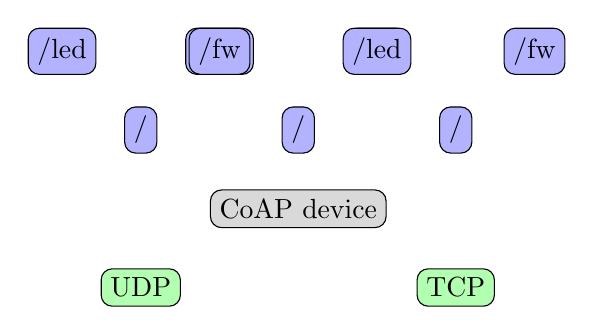
\begin{tikzpicture}
		\node[host] (host) at (0, 0) {CoAP device};
		\node[proto] (udp) at (-2, -1) {UDP};
		\node[proto] (tcp) at (2, -1) {TCP};

		\node<1,3>[res, above of=host] (x-root) {/};
		\node<1,3>[above of=x-root] (x-head) {};
		\node<1,3>[res, left of=x-head] (x-led) {/led};
		\node<1,3>[res, right of=x-head] (x-fw) {/fw};

		\node<2>[res, above of=host, above of=udp] (u-root) {/};
		\node<2>[above of=u-root] (u-head) {};
		\node<2>[res, left of=u-head] (u-led) {/led};
		\node<2>[res, right of=u-head] (u-fw) {/fw};

		\node<2>[res, above of=host, above of=tcp] (t-root) {/};
		\node<2>[above of=t-root] (t-head) {};
		\node<2>[res, left of=t-head] (t-led) {/led};
		\node<2>[res, right of=t-head] (t-fw) {/fw};
	\end{tikzpicture}

	\raggedright

	\only<1>{
		\vspace{3em}

		\footnotesize Not just TCP/UDP: (D)TLS and WebSockets are specified; there are drafts for SMS, serial lines and Bluetooth, and ideas for QUIC, possibly via TAPS.
	}

	\only<2>{
		\texttt{coap+tcp://[2001:db8::1]/led} $\not=$ \texttt{coap://[2002:db8::1]/led}

		\bigskip

		Server MAY do this, client MUST NOT assume it.
		See \texttt{http} vs. \texttt{https}.
	}

	\only<3->{
		\texttt{coap+tcp://[2001:db8::1]/led} $\stackrel{?}{:=}$ \texttt{coap://[2002:db8::1]/led}

		\bigskip

		\begin{itemize}
			\item ``aliasing'' -- gernerally discouraged on URIs.
			\item Multiple cache entries.
			\item What does identity mean for, say, block-wise operation?
			\item What does identity mean security?
			\item Breaking change.
		\end{itemize}
	}
\end{frame}

\begin{frame}{Proposed mechanism: We have the runtime parts}\large
	\center
	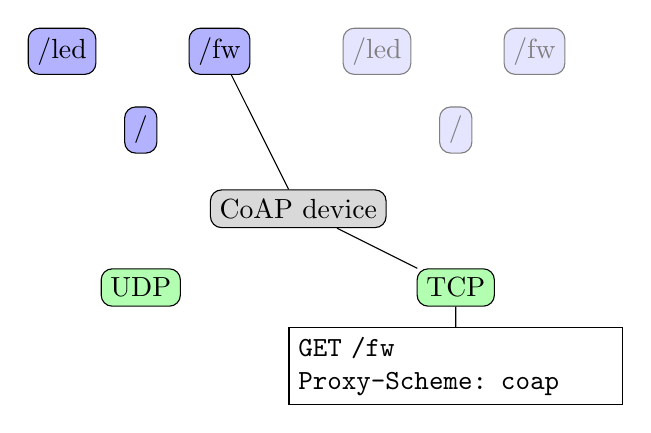
\begin{tikzpicture}
		\node[host] (host) at (0, 0) {CoAP device};
		\node[proto] (udp) at (-2, -1) {UDP};
		\node[proto] (tcp) at (2, -1) {TCP};

		\node[res, above of=host, above of=udp] (u-root) {/};
		\node[above of=u-root] (u-head) {};
		\node[res, left of=u-head] (u-led) {/led};
		\node[res, right of=u-head] (u-fw) {/fw};

		\node[nonres, above of=host, above of=tcp] (t-root) {/};
		\node[above of=t-root] (t-head) {};
		\node[nonres, left of=t-head] (t-led) {/led};
		\node[nonres, right of=t-head] (t-fw) {/fw};

		\node[req,below of=tcp,text width=4cm] (req) {\texttt{GET /fw}\\\texttt{Proxy-Scheme: coap}};

		\draw (req) -- (tcp) -- (host) -- (u-fw);
	\end{tikzpicture}

	\raggedright

	The option is already there,
	and has the right meaning:

	\bigskip

	RFC 7252 Section 6.5 gives \texttt{coap://[2001:db8::1]/fw} -- the intended URI.

	\bigskip

	``Being a proxy'' is a big word -- it's really just processing that option.
\end{frame}

\begin{frame}{Proposed mechanism: We need discovery}\large
	\center
	\begin{tikzpicture}
		\node[res, above of=host, above of=host] (x-root) {/};
		\node[above of=x-root] (x-head) {};
		\node[res, left of=x-head] (x-led) {/led};
		\node[res, right of=x-head] (x-fw) {/fw};

		\node[proto, right of=x-fw, right of=x-root] (x-coaptcp) {TCP};

		\draw[-stealth] (x-root) -- (x-fw);
		\draw[-stealth] (x-root) -- (x-led);
		\draw[-stealth] (x-root) -- node [below] {proxy} (x-coaptcp);
	\end{tikzpicture}

	\bigskip

	``the proxy is'' 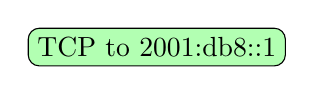
\begin{tikzpicture}[baseline=-1mm]\node[proto] {TCP to 2001:db8::1};\end{tikzpicture} $\mapsto$ ``proxy identified as'' 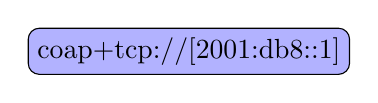
\begin{tikzpicture}[baseline=-1mm]\node[res] {coap+tcp://[2001:db8::1]};\end{tikzpicture}

	\bigskip

	\raggedright
	\texttt{</fw>;rt="tag:...:suit"}{\color{gray}\texttt{;rel=hosts;anchor="/"}}\texttt{,}\\
	\texttt{<coap+tcp://[2001:db8::1]/>;rel=}{\color{blue}\texttt{has-proxy}}{\color{gray}\texttt{;anchor="/"}}

	\bigskip

	\begin{block}{Goals (1-2/5)}
		\textbf{Enablement} Inform clients of the availability of other transports of servers.

		\textbf{No Aliasing} Any URI aliasing must be opt-in by the server. Any defined mechanisms must allow applications to keep working on the canonical URIs given by the server.
	\end{block}
\end{frame}

\begin{frame}{Security Considerations}
	\color{gray}
	\Huge Just As With Any Proxy.

	\bigskip

	\footnotesize OK, there's more in the text, but that's the gist.
	\large

	\vspace{2cm}

	\color{black}
	\begin{itemize}
		\item Any requirements on connecting directly apply also on the connection through a proxy.
		\item Proxies that do not have the relevant precise credentials are out of scope.
		\item Users worrying about traffic misdirection can decide to only use a proxy statement if it comes from an authoritative source.
	\end{itemize}
\end{frame}

\begin{frame}{Is this enough?}
	\pause
	Maybe.

	\vspace{3cm}

	\pause
	Proxy may be provided by anyone (not ruled out so far, but not described either).
	
	\bigskip

	And we still send 5 bytes per request\ldots
\end{frame}

\begin{frame}{Proxy interaction}\large
	\begin{block}{Goals (4-5/5)}
		\textbf{Proxy usability} All information provided must be usable by aware proxies to reduce the need for duplicate cache entries.

		\textbf{Proxy announcement} Allow third parties to announce that they provide alternative transports to a host.
	\end{block}

	Proxies see a single resource. Proxies may use it to pick their upstream.

	\bigskip

	External components (e.\,g. a Resource Directory) can state that they provide proxying services.

	Whether a client uses them depends on client's security requirements;
	as a minimum, application and transport layer security must not deteriorate.
	(Generally trivial with OSCORE and out of scope for (D)TLS).
\end{frame}

\begin{frame}{Eliminating per-request overhead}\Large
	\begin{block}{Goals (3/5)}
		\textbf{Optimization} Do not incur per-request overhead from switching protocls. This may depend on the server's willingness to create aliased URIs.
	\end{block}

	\bigskip

	\mbox{
	\texttt{<coap+tcp://[2001:db8::1]/>;rel=}{\color{blue}\texttt{has-unique-proxy}}{\color{gray}\texttt{;anchor="/"}}
	}

	\bigskip

	Request can go to \texttt{coap+tcp://} on the wire; application still think in terms of \texttt{coap://}. Looks like aliasing, but that's a matter of perspective (SCHC?).

	\bigskip

	\footnotesize Also answers: ``Do I have to send the Uri-Host option?''
\end{frame}

\begin{frame}{Eliminating per-request overhead: Security}\Large
	Open issue: Potential confusion about intended resource.

	\bigskip

	Possible solution:
	Accept unique-proxy statement only when coming from authoritative resource.

	\bigskip

	(No big loss: Third party proxies are generally non-unique anyway).
\end{frame}

\begin{frame}{Take-home message}\Large 
	\begin{itemize}
		\item It can probably be just this simple.
		\item No URI aliasing introduced in applications.
	\end{itemize}

	\vspace{2cm}

	Questions? Comments? Way forward?
\end{frame}

\begin{frame}{Backup slide / FAQ}
	\setlength{\parskip}{0.3em}
	\textit{Didn't we want to do this with DNS?}

	We\footnote{Whoever wants to use it will need to volunteer as coauthor.} still can, just need to phrase the equivalent statements in DNS.

	Straw man for ``\texttt{coap://device.example.com} has CoAP-over-TCP running on port 1234'':

	\texttt{\_has-coap-proxy.\_tcp.device.example.com SRV 0 0 device.example.com 1234}
	\texttt{device.example.com AAAA 2001:db8::1}

	\bigskip

	\textit{How does this relate to HTTP's \texttt{Alt-Svc}?}

	Generally similar; links instead of headers (as common in CoAP), and no need for protocol-id because we have schemes already.

	\bigskip

	\textit{How does this (esp. security for unique proxies) relate to CoRAL?}

	Yes.
\end{frame}

\end{document}
